
\documentclass[letterpaper,times]{IONconf/IONconf}

\usepackage{amsmath}
\usepackage{graphicx}
\usepackage{multirow}
\usepackage{float}
\usepackage[ruled,vlined]{algorithm2e}
\SetArgSty{textnormal}

\title{On SBAS Authentication with OTAR Schemes}
\author{Jason Anderson, Sherman Lo, Andrew Neish, Todd Walter}

\begin{document}

	\maketitle

\begin{abstract}
	Herein we delineate a complete Satellite-Based Augmentation System (``SBAS'') authentication scheme, including over-the-air re-keying (``OTAR''), that uses Elliptic Curve Digital Signature Algorithm (``ECDSA'') and Timed Efficient Stream Loss Tolerant Authentication (``TESLA'') without using the Quadrature (``Q'') channel.
	This scheme appends two new message types (''MT'') to the SBAS scheduler without overburdening the SBAS message schedule.
	We take special care to make our scheme (1) meet appropriate security requirements to prevent and deter spoofing; (2) compatible with existing cryptographic standards; (3) flexible, expandable, and future proof to different cryptographic and implementation schemes; and (4) backward compatible with legacy receivers.
	The scheme accommodates a diverse set of features, including authenticating core-constellation ephemerides.
	The scheme requires loose time synchronization between the receiver and the provider, and we assert reasonable mitigation strategies to prevent attacks to that assumption.
	This work also discusses the SBAS provider and receiver machine state and startup, including aircraft that traverse differing SBAS coverage areas.
	We test our scheme with existing SBAS simulation and analysis tools to show negligible effects on SBAS availability and continuity requirements.
\end{abstract}

\section{Introduction} \label{sec:introduction}

	In this work, we delineate a complete Satellite-Based Augmentation System (the service itself, ``SBAS'') authentication scheme, including over-the-air re-keying (``OTAR'') and then discuss how this proposed scheme meets necessary security levels and desirable traits to SBAS stakeholders, such as backward compatibility, data efficiency, and quick time to authenticated first fix (``TFAF'').
	Moreover, it is expandable to additional stakeholder feedback.
	This work addresses the complete authentication scheme design, including connecting receiver hardware requirements to maintenance schedules, key updates, and scheme maintenance, and uses a full-stack Monte-Carlo SBAS simulation to test and evaluate the scheme's performance.

	Satellite-Based Augmentation Systems (the several international systems together, ``SBASs''), such as the United States' Wide-Area Augmentation System (``WAAS'') among other international equivalents, have become integral to the Global Navigation Satellite System (``GNSS'') for civilian aviation use.
	International parties that choose to implement an SBAS (each a ``Provider'') use listening stations around their service volume to assess GNSS satellite positioning data and then broadcast corrections widely via geostationary satellites.
	This information includes wide-area GNSS differential corrections and GNSS satellite health and integrity.
	Like most GNSS core-constellation signals, the SBAS signal is open and susceptible to spoofing, and with its ubiquitous use in civilian aviation, SBAS should be augmented with spoofing resistant capabilities to ensure continued civilian aviation safety.
	Providers agree to share a common SBAS message standard.
	This work pertains to how the SBAS message standard could be augmented to provide an authenticated service resistant to spoofing.

	SBAS is primarily a data service.
	It broadcasts data that assists GNSS users.
	Therefore, appending additional cryptographic data to the SBAS data is a natural way to authenticate the SBAS data for civil users.
	Additional SBAS broadcast messages could deliver cryptographic signatures and key values to users.
	Using the mathematical primitives underlying cryptographic authentication methods, users could assert that only a Provider could have generated the SBAS data and the accompanying authenticating psuedorandom data.
	In this work, we call the authenticating data ``signatures'', and signatures, together with the associated key data, either ``authenticating psuedorandom data'' or ``OTAR Segment'', referring to the cryptographic pseudorandom data itself or the chunks separated for transmission to receiver, respectively.
	We call this data authenticating psuedorandom data because the data is not human-readable nor predictable (without private secrets).
	The security of the authenticating psuedorandom data assumes that (1) Provider exclusively holds certain identifying information secret and (2) there exist no {\em known} efficient algorithms that can generate the authenticating psuedorandom data without the identifying information held secret.
	If the identifying information (e.g., keys) is leaked, that information is called compromised and must be revoked.
	If an efficient algorithm is discovered, the relevant cryptographic primitives are called broken, and those primitives must be replaced.

	Using cryptographic authentication methods poses challenges to SBAS.
	The main challenge is delivering the authenticating psuedorandom data via SBAS, given the data-bandwidth constraints.
	Since SBAS is an open signal, SBAS authentication security must rely on asymmetric cryptographic algorithms to provide authentication, such as Elliptic Curve Digital Signature Algorithm (``ECDSA'').
	Herein, wherever we specify ECDSA, we could use another similar asymmetric cryptographic algorithm (e.g., EC-Schnorr); however, we will specify ECDSA without losing generality for concreteness, noting that certain parameters and characteristic security strengths listed here would be different if not using ECDSA.
	A single ECDSA signature requires 512-bits to achieve the standard 128-bit security level with ECDSA, which dwarfs the 216 data bits allowed per SBAS message.

	Some prior art has suggested using the Quadrature (``Q'') channel to deliver the authenticating psuedorandom data \cite{todd-pki-scheme, other_schemes}; however, those solutions would require power from the current use of the In-phase (``I'') channel.
	Using the Q channel would strain the availability and continuity of SBAS systems at coverage area boundaries, which is undesirable to SBAS stakeholders.
	Some prior art has suggested using a combination of ECDSA with another algorithm called Timed Efficient Stream Loss Tolerant Authentication (``TESLA'') \cite{Neish_Dissertation, gal-os-tesla} since it provides more efficient use of authenticating psuedorandom data and is loss-tolerant.
	TESLA uses a delayed-release mechanism to authenticate data with less authenticating psuedorandom data than that required by ECDSA; however, it requires that Provider and a user be loosely time-synchronized \cite{perrig2005timed}.
	SBAS cannot exclusively use TESLA: TESLA must be used in tandem with ECDSA to achieve authentication security.
	In this work, we establish the following relationship between the proposed TESLA-ECDSA scheme: TESLA authenticates the SBAS messages themselves, and ECDSA authenticates SBAS's use of TESLA as periodic {\em maintenance}.
	The prior art has specified that TESLA and ECDSA scheme parameters required to achieve authentication; however, it has largely not addressed the maintenance and maintenance requirements, such as how best to perform OTAR.
	This work addresses the main challenge by suggesting a more efficient authentication maintenance scheme without using the Q channel.
	Moreover, this work leverages specific features of TESLA scheme to assert security efficiently \cite{chain-security} and allows additional features relevant to SBAS stakeholders.

	Another challenge lies with receiver computational considerations.
	Some prior art has explored how TESLA and ECDSA computations would fare with use in the GNSS, SBAS, and smartphone context \cite{tesla-cpus}.
	TESLA often requires a more intense, one-time startup hashing computation upon receiver start and minimal hashing operations during standard operation.
	We note that modern commodity electronics perform these operations often and often include hardware-specific acceleration in their chips to increase computational efficiency and allow parallelism.
	Therefore, we expect that if these methods burden current receivers, receiver manufacturers could augment their chips at a minimal cost to maintain desirable computational loads.

	Prior art suggested appending a single message type (``MT'') to SBAS for authentication and its maintenance\cite{Neish_Dissertation}.
	It suggests that SBAS sends this MT every six messages and that this MT delivers 190-bits of TESLA authentication data and 26-bits for the scheme's maintenance.
	While the scheme requires a steep authentication-message delivery frequency, it does not overburden the SBAS MT schedule.
	We modify this work by appending another MT to SBAS to replace the 26-bits mentioned above dedicated for maintenance.
	We design our proposed additional MT to be modular with the exclusive purpose of delivering all authenticating psuedorandom data related to the scheme's maintenance.
	This design allows for reasonable TFAF requirements.
	It is agnostic to the ECDSA and TESLA scheme parameters; therefore, it requires minimal changes in the event of cryptographic primitive breakage.
	Moreover, it scales well with increases to the security level requirements and is flexible and future-proof to anticipated feedback from Providers and SBAS stakeholders.

	To evaluate the proposed method against prior art, we implement a full-stack SBAS simulation of our design by augmenting an existing SBAS simulation tool called Matlab Algorithm Availability Simulation Tool (``MAAST'')\cite{MAAST}.
	MAAST has been used to evaluate SBAS design before and provides Monte-Carlo simulation results to evaluate how our design performs under message loss over the WAAS coverage area.
	The tool shows that our proposed design outperforms Key Performance Indicators (each a ``KPI''), such as TFAF, time to authentication per message, and robustness to message loss.

	With TESLA's use, Provider and any users must be loosely time-synchronized, which poses an interesting Catch-22 situation since GNSS provides the time.
	Therefore, our scheme must also describe its resistance to a Replay Attack.
	A Replay Attack is where a spoofer listens and then replays messages at a slightly delayed rate.
	After some time, the spoofer-induced time delay allows the spoofer to violate the loosely-time synchronized assumption and break the TESLA scheme.
	There are ways from the prior art by which receivers can establish trust in GNSS ranging signals\cite{Psiaki2016,Fernandez-Hernandez2018}; however, GNSS ranging signals are not yet rigorously authenticated with cryptography.
	Some prior art has described how an onboard receiver clock could be used to detect such an attack, given clock uncertainty\cite{time_sync_paper}.
	This work extends that work of prior art by discussing how onboard clocks, external clocks, and maintenance conditions can be used to mitigate Replay Attack threats.

	\subsection{ECDSA} \label{sub:ecdsa}

		ECDSA is a standardized asymmetric authentication protocol.
		There are details not mentioned in the following summary description of ECDSA, so for a more precise definition, we refer the reader to widely available detailed definitions in cryptographic literature or the internet.
		The protocol specifies a signing function and a verifying function.
		Let $n$ be the security level of an instance of the protocol, which linearly describes the required computation to {\em exhaustively} break the instance.
		Provider generates a secure random $2n$-bit integer for long-term use as a secret private key.
		Provider then derives a $2n$-bit integer from the private key and distributes it to receivers as the public key.
		Provider uses the signing function, with the secret private key, to derive signatures on messages.
		Each signature is a 2-tuple of $2n$-bit integers, for a total of $4n$ bits.
		Receivers use the verifying function, with the public key and signatures, to assert that the private key holder generated the message and signature.
		Since the protocol is secure, there is no {\em known} efficient algorithm that can compute the private key given the public key nor compute the signature on a message without the private key.
		The protocol assumes that the receiver trusts the public key as from Provider.
		The protocol is not loss-tolerant: if a single bit of a signature or message is lost, the protocol will fail to verify.

	\subsection{TESLA} \label{sub:tesla}

		TESLA is an authentication protocol that allows a receiver to authenticate messages from Provider when used in tandem with other asymmetric authentication protocols.
		This protocol poses several advantages over a purely asymmetric system relevant to GNSS and SBAS systems.
		First, the protocol requires less authenticating psuedorandom data to authenticate messages from Provider.
		Second, the protocol is loss-tolerant.
		Third, the receiver authentication computation is less strenuous.
		Figure~\ref{fig: TESLA Diagram} provides a conceptual diagram of the TESLA description that follows.
		Algorithms~\ref{alg: TESLA provider} and~\ref{alg: TESLA receiver} describe the protocol more concretely.
		\begin{figure}%\label{fig: TESLA Diagram}
			\centering
			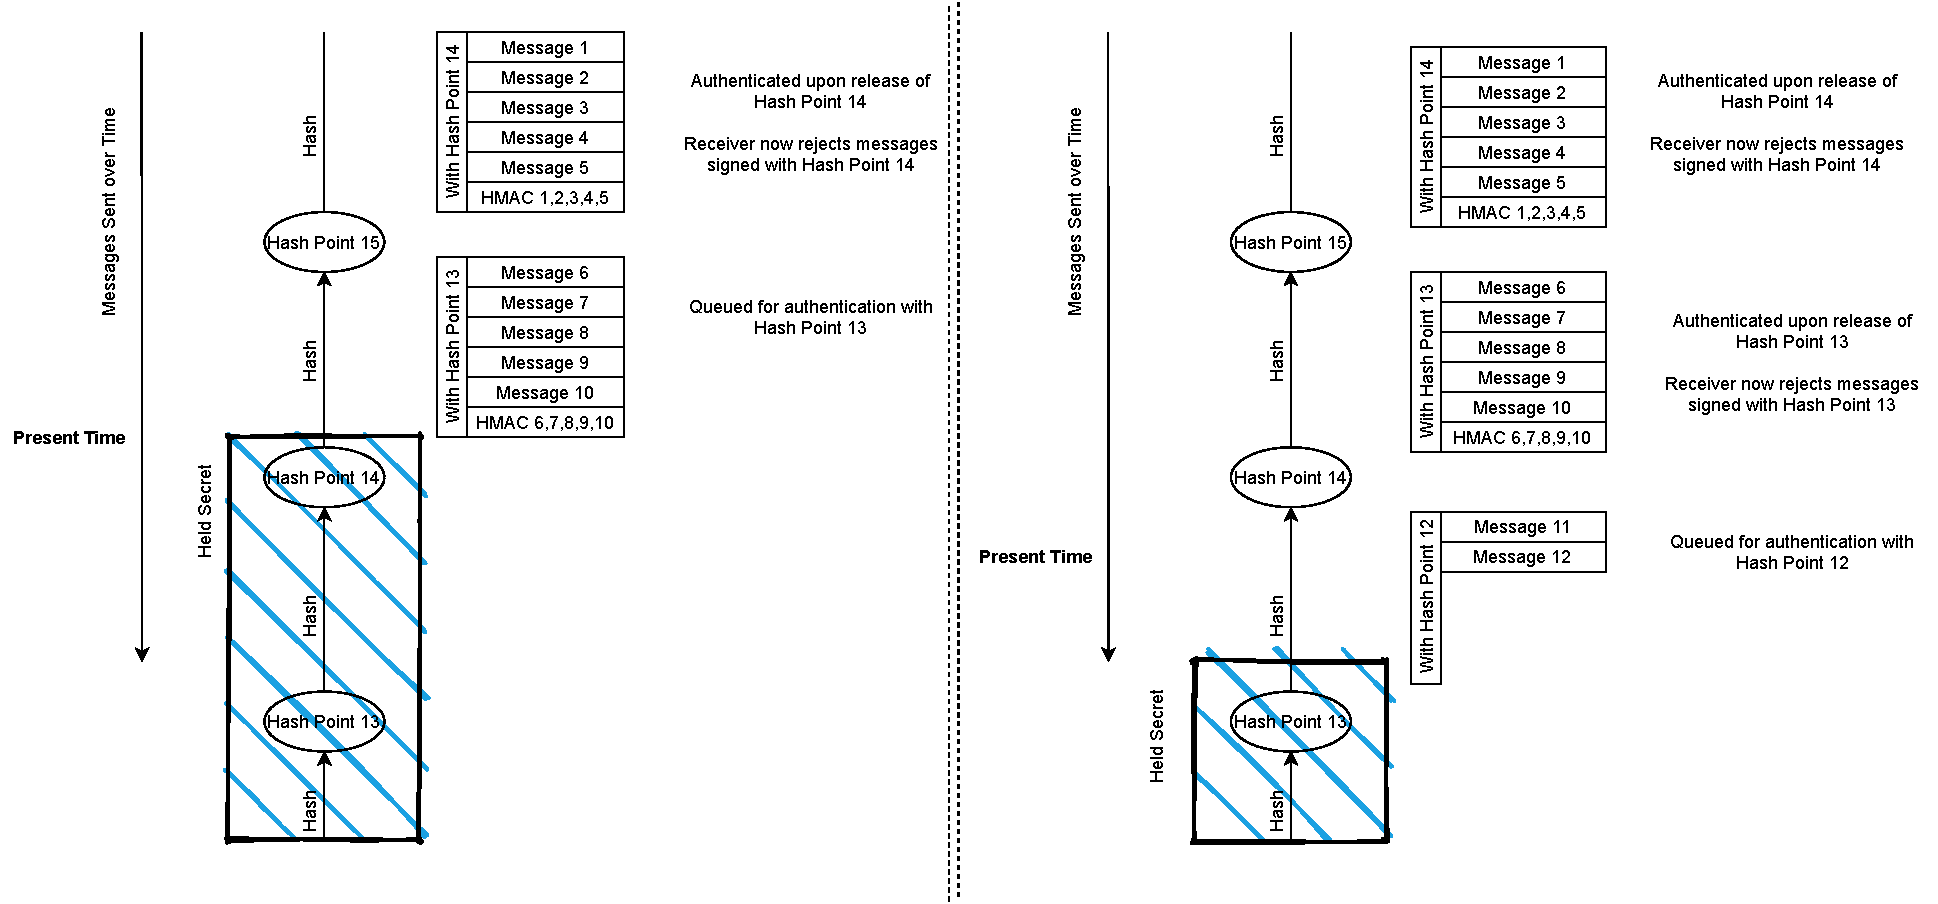
\includegraphics[width=\linewidth]{fig/TESLADiagram.pdf}
			\caption{
				Conceptional diagram of TESLA that demonstrates the delayed-release key secrecy schedule.
				The right section of the diagram follows the left section of the diagram in time.
				The diagonally cross-hashed box notes information held secret by Provider.
				The box recedes each time a Hash Point is released.
			}
			\label{fig: TESLA Diagram}
		\end{figure}

		TESLA uses only a single cryptographic primitive: a cryptographically secure hash function.
		In this proposal, we select a salted SHA-256, truncated to the left-most 128-bits (herein, the ``Hash Function'' or $\textrm{H}(\cdot)$), so we describe the TESLA protocol concretely using our selection without loss of generality.
		We truncate Hash Function output to the 128 most-significant bits to make 128-bit integers.
		Since the audience of this work are experts in navigation, we use geometric terms {\em path} and {\em point} instead of {\em key chains} and {\em key} and describe TESLA with the geometry of a {\em one-way path}.
		Let each 128-bit integer be called a Hash Point, and let a collection of Hash Points {\em consecutively} related via the Hash Function be a Hash Path.
		Non-consecutive Hash Points further along the Hash Path relate via repeated application of the Hash Function.
		Since the Hash Function is secure, there is no {\em known} efficient algorithm that can compute the input Hash Point to the Hash Function that yields a specific output Hash Point.
		Herein, we call that input Hash Point the preimage Hash Point of that output Hash Point.
		In other words, it is trivially easy to compute the output Hash Point of the Hash Function given the preimage Hash Point, but one can only use exhaustive search to find any preimage Hash Point.
		It is a {\em one-way} path.
		The domain of 128-bit integers, together with a randomized 128-bit salt inclusion to the Hash Function, make precomputation attacks (also called Rainbow Table Attacks) infeasible with modern supercomputers because it meets 128-bit security.
		Our use of the term Hash Point also serves to avoid confusion with the overloaded use of ``key'' among TESLA and ECDSA.
		Authentication private and public keys relate to ECDSA, and many keys will derive from TESLA Hash Points to achieve the required authentication data bandwidth efficiency.

		To use a Hash Path to authenticate messages via TESLA, Provider computes a Hash Path derived from a {\em random} starting Hash Point and holds that Hash Path secret.
		Provider broadcasts the last Hash Point along the Hash Path (herein, the "Hash Path End") together with an ECDSA signature derived therefrom.
		Receivers assert the Hash Path End as authenticated with the ECDSA signature.
		Provider uses the secret preimage Hash Point to the Hash Path End to derive HMAC keys to send symmetric authentication signatures along with the standard message set.
		We propose using keyed-hash message authentication codes that use the Hash Function as its primitive for message signatures (the function, ``HMAC'', and the HMAC signatures themselves, ``HMACs''). 
		We will continue to describe the protocol concretely using our selection without loss of generality.
		We truncate the HMACs to the left most bits to fit the HMACs in SBAS messages.
		Providers and receivers agree on a schedule where Provider will (1) stop using the preimage Hash Point of the Hash Path End to authenticate messages, (2) broadcast that preimage Hash Point for receivers to authenticate messages, and (3) use the next preimage Hash Point along the Hash Path to authenticate new messages.
		Once a particular preimage Hash Point is broadcast, receivers cannot accept new signatures received derived therefrom.
		Since the HMACs were received when a specific preimage Hash Point was known only to Provider, Provider must have generated the messages.
		Each time Provider releases a Hash Point, Provider moves backward one Hash Point along its secret Hash Path to derive new HMACs.
		Given the Hash Function's security, the Hash Point along the Hash Path before the released Hash Point is still secret, and so it becomes the new HMAC key for the next set of messages.
		The authentication security along the Hash Path hinges on (1) the security of the Hash Function and (2) that Provider and receiver are loosely time-synchronized.

		To complete authenticating security, TESLA must be used in tandem with an asymmetric authentication protocol.
		TESLA is secure along the Hash Path length; however, Hash Paths are finite and must be generated periodically.
		An asymmetric authentication protocol must sign the Hash Path End, the first Hash Point known to the receiver.
		In other words, for every Hash Path generated by Provider, Provider must use an asymmetric signature to ensure authentication security along the entire Hash Path.
		Moreover, Provider and receiver must be loosely time-synchronized, which poses a Catch-22 problem since GNSS and SBAS Providers provide the time.
		This provokes the question of why use TESLA at all and not just use only an asymmetric protocol.
		Later in this work, we will show that using TESLA has better loss-tolerant properties, requires less authenticating psuedorandom data, and the time-synchronization problem can be accounted for.

\section{SBAS Authentication Scheme Definition} \label{sec:sbas_authentication_scheme_definition}

	This SBAS authentication proposal proposes appending two message types to the schedule (herein, ``MT50'' and ``MT51'').
	MT50 is used to authenticate the actual SBAS messages via the TESLA protocol.
	MT51 is used to (1) authenticate the Hash Path Ends via ECDSA as Provider uses series of Hash Paths in its standard operation, and (2) to provide OTAR and perform system-level maintenance of the cryptographic authentication scheme.
	Here follows in this Section~\ref{sec:sbas_authentication_scheme_definition} precise definitions of our proposed SBAS authentication scheme.
	Sections~\ref{sec:tesla_design_methodology} and~\ref{sec:otar_design_methodology} provides explanations and reasoning for our proposed definitions.
	While the definitions presented here are for the L5 signal, given the spare bits remaining in each definition, this scheme will also work for the L1 signal by modifying the preambles (noted with reserved bits in definitions).

	\subsection{ECDSA Key Structure} \label{sub:ecdsa_key_structure}

		We propose a two-level ECDSA key structure, as suggested \cite{Neish_Dissertation}.

		Level-1 keys will be 256-bit ECDSA keys managed internationally by a trusted Certificate Authority (``CA'').
		Each level-1 key will be in use for 100 weeks.
		CA shall compute a large number of level-1 keys for use in the perpetual future and then encrypt each key individually via AES-128 with different AES encryption keys (one per level-1 key) held secret by CA.
		CA will distribute the AES-ciphertext to receiver manufacturers.
		Receivers will come preloaded with the collection of 512-bit public keys, encrypted with 128-bit keys via AES-128.
		As level-1 keys expire, CA will distribute the keys to decrypt the AES-ciphertext, one at a time, for Provider to distribute via MT51.
		As the receiver receives the key to decrypt its onboard AES-ciphertext, it will update its current level-1 ECDSA public key.
		Each level-1 public key will be a 512-bits, and any signature derived therefrom will be a 1024-bits.

		Level-2 keys will be 128-bit ECDSA keys managed by Provider.
		Each level-2 key will be in use for ten weeks.
		For a new level-2 key, Provider will generate a secure-random private ECDSA key and its associated public key.
		Provider will submit the new public key to CA for a signature from CA's current level-1 key.
		Provider will then distribute that public key and the associated authenticating signature over SBAS.
		The receiver receives a new level-2 public key and the authenticating signature, verifying the received new level-2 public key with the associated decrypted level-1 public key.

		Provider will use its level-2 keys to authenticate TESLA Hash Path Ends, and keys derived from the TESLA Hash Paths will be used to authenticate the bulk of SBAS messages with HMACs.
		For all levels, the authenticating psuedorandom data delivered will accompany data (e.g., SBAS message preamble, MT, other data) that must be sent per the definitions below.
		A particular signature must derive from the entire SBAS message(s) used to deliver that particular key.
		Concretely, when a level-1 key authenticates a level-2 key, the level-1 signature must derive from the entire set of messages used to deliver the level-2 key and the accompanying key expiration time. 
		In other words, the level-1 signature must derive from the complete messages containing overhead data, not just the level-2 key itself.
		If this does not happen, then the accompanying data, especially the key expiration time, will not be secured by the cryptographic primitives.

	\subsection{TESLA Hash Path and HMAC Keys} \label{sub:tesla_hash_path}

		Each TESLA Hash Path will be used over one week.
		Provider will generate an entire Hash Path before its actual use and then broadcast the Hash Path End, signed by the current level-2 ECDSA key via MT51.
		Each Hash Point, except the Hash Path End, will be associated with at least five HMAC keys that will authenticate at least five messages with HMAC, depending on the number of iterations of Equation~\eqref{eq: key}.
		Therefore, a Hash Path will include 100801 Hash Points: one for each sixth second for the week and then the Hash Path End.

		To generate a Hash Path $P$, Provider will derive a secure random 128-bit salt $S^P$ from level-2 ECDSA authentication, as described in Section~\ref{subsub:ecdsa_salt}.
		Let the Hash Points of $P$ be denoted $p^P_i$, and let $t_i$ be the time at which Provider publicly releases $p^P_i$ via broadcast.
		Here, $t_i$ is an integer time (e.g., time in seconds since the GPS epoch).
		We propose Equation~\eqref{eq: hash path} define the Hash Path where $||$ denotes bit concatenation and $\oslash$ denotes integer division.
		\begin{equation}
			p^P_{i+1} = \textrm{H} \left(p^P_i || S^P || (t_i \oslash 6) \right) \label{eq: hash path}
		\end{equation}
		The purpose of the integer division is explained in Section~\ref{subsub:time_counter}.
		We propose a left-most 16-bit truncated signature from HMAC authenticates each SBAS message delivered via MT50.
		The key $k_j$ for each message $m_j$ will be according to Equation~\eqref{eq: key}, and the signature $s_j$ derived therefrom will be according to Equation~\eqref{eq: signature}.
		$t_j$ is the integer time of the authenticated message's broadcast and receipt.
		PRN is the pseudorandom code associated with the broadcasting geostationary satellite.
		Frequency is the frequency band of the particular transmission (e.g., L1 or L5).
		We discuss the necessity of the concatenation and HMAC operations of Equation~\eqref{eq: key} in Sections~\ref{sub:tesla_efficiency} and~\ref{sub:tesla_security}.
		Equation~\eqref{eq: key} ensures that each HMAC for each message from each satellite has its own key. 
		\begin{align}
			k_j &= \textrm{HMAC}(p^P_i, t_j || \textrm{PRN} || \textrm{Frequency} \label{eq: key}) \\
			s_j &= \textrm{HMAC}(k_j, m_j) \label{eq: signature}
		\end{align}
		The output of Equation~\eqref{eq: signature} is truncated to the 16 most-significant bits.
		We note that Equations~\eqref{eq: hash path} and~\eqref{eq: key} use a concatenation operation because the input data is less than 512-bits, the block size for the selected Hash Function.
		These operations would need to be modified if the input data were ever larger than 512-bits.

		Section~\ref{sub:procedures} and Algorithms~\ref{alg: TESLA provider} and~\ref{alg: TESLA receiver} concretely describe how Provider and receivers should authenticate, queue, and cache, to verify messages.

	\subsection{MT50} \label{sub:mt50}

		Table~\ref{tab: mt50} provides our proposed definition of MT50 with the bit allocations.
		Provider will send an MT50 at a cadence of every six messages.
		The delayed key release to authenticate messages means that messages will be authenticated between 7 and 11 seconds after their broadcast.
		Provider will set the cadence of integrity messages to always immediately proceed MT50s to minimize integrity message authentication time.
		If the receiver is not able to authenticate a message because of a lost MT50, it generally disregards that message (messages that inform receivers to decrease the level or trust or to not use the service do not need to be disregarded).
		Within the message definition, there are five 16-bit HMACs and one 128-bit Hash Point.
		At the receiver receipt of an MT50, the included five HMACs correspond to the previous messages with a secret Hash Point known only to Provider at message sending time.
		The included 128-bit Hash Point corresponds to the HMACS included in the {\em previous} MT50 message sent 6 seconds earlier.
		Figure~\ref{fig: MT50 Schedule} provides a conceptual diagram of the delayed Hash Point key release.

		\begin{table}%\label{tab: mt50}
			\center
			\begin{tabular}{|c|c|c|c|c|c|c|c|c|c|c|} \hline
				Preamble & MT & Reserved & HMAC1 & HMAC2 & HMAC3 & HMAC4 & HMAC5 & Hash Point & Spare & CRC \\ \hline
				4 & 6 & 4 & 16 & 16 & 16 & 16 & 16 & 128 & 4 & 24 \\ \hline
			\end{tabular}
			\caption{Bit Allocation for proposed MT50. Per SBAS definitions, there are 250 bits per message.}
			\label{tab: mt50}
		\end{table}

		\begin{figure}%\label{fig: MT50 Schedule}
			\centering
			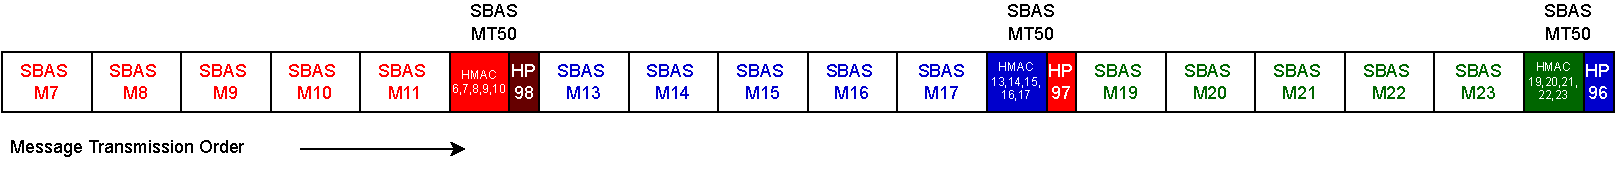
\includegraphics[width=0.5\linewidth]{fig/MT50Schedule.pdf}
			\caption{
				A conceptual diagram of how consecutive MT50 messages relate to each other.
				The colors correspond to a specific Hash Point along the Hash Path. Each MT50 includes the HMACs of the five previous messages, and the Hash Point used for the HMACs sent six messages earlier.
			}
			\label{fig: MT50 Schedule}
		\end{figure}

		Per the SBAS specifications, in the event of a GNSS integrity alert, an alert message must be sent by Provider four messages in a row.
		Therefore,  occasionally an alert message will take priority over an MT50.
		The salted Hash Function described in Equation~\eqref{eq: hash path} accommodates small perturbations to the schedule resulting from alert messages, see Section~\ref{subsub:time_counter} and Figure~\ref{fig: alert schedule}.
		Even with an MT50 delay, each MT50 must sign the messages it would have signed without an alert, see Section~\ref{sub:tesla_security}.

	\subsection{MT51} \label{sub:mt51}

		In this work, we provide two MT51 definitions: MT51-A and MT51-B.
		The A and B versions represent opposite ends of a spectrum on which a final MT51 would lie.
		MT51-A and MT51-B are alternatives to each other, i.e., they would not be used by Provider simultaneously in the same SBAS.
		The difference between MT51-A and MT51-B is bits devoted to (1) the OTAR Payload Segment and (2) meta-data describing how to interpret the OTAR Payload Segment of a particular MT51.
		MT51-A is bare bones and featureless; whereas, MT51-B contains features that could be relevant to the SBAS stakeholders.
		We refrain from specifying which features should be incorporated, deferring until all SBAS stakeholders have had their considerations heard.
		If SBAS stakeholders do not care for the additional features described later with MT51-B, then the final design should be MT51-A.
		If SBAS stakeholders desire some or all of the additional features of MT51-B, then the final design should be MT51-B.
		Given the flexibility of the MT51 design (as discussed later), a final design would lie somewhere in between MT51-A and MT51-B.
		While this section provides the MT51 definitions for the MT51 spectrum ends, Section~\ref{sec:otar_design_methodology} discusses how to reason finding the right balance.
		
		Since MT51-A has less meta-data, more message data is dedicated to the OTAR Payload Segment, decreasing the number of unique MT51s required to OTAR.
		Since less messages are required to OTAR with MT51-A, we expect better continuity, availability, and TFAF results.
		We will show that feature-rich MT51-B is able to meet our requirements and not burden the SBAS schedule.
		Since MT51-B already meets the KPIs and given the academic context of this work, we focus on MT51-B to study the feature potential to SBAS stakeholders.
		
		Table~\ref{tab: mt51-a} provides our proposed definition of MT51-A with bit allocations, and Tables~\ref{tab: mt51-b}~and~\ref{tab: meta-data} together provide our proposed definition of MT51-B with bit allocations.
		Provider must broadcast MT51 messages approximately every 1 in 30 messages for MT51-A and every 1 in 18 messages for MT51-B, see Section~\ref{sub:mt51_schedule_frequency}.
		These messages do not have to be sent on a rigid schedule and can be sent in the extra space within the current SBAS schedule.

		\begin{table}%\label{tab: mt51-a}
				\center
				\begin{tabular}{|c|c|c|c|c|c|} \hline
				\multicolumn{6}{|c|}{MT51-A Bit Allocation} \\ \hline
					Preamble & MT & Reserved & Segment Number & OTAR Segment & CRC \\ \hline
					4 & 6 & 4 & 5 & 207 & 24 \\ \hline
				\end{tabular}
				\caption{
					Bit allocation proposed for MT51-A at 250 bits per message. 
					The Authentication Stack, defined in Section \ref{sub:procedures}, is composed of a total 2048 bits, requiring receipt of the ten unique messages to OTAR.
					Since each segment is cryptographic psuedorandom, a segment number must accompany each OTAR segment.
				}
				\label{tab: mt51-a}
			\end{table}

		\begin{table}%\label{tab: mt51-b}
			\center
			\begin{tabular}{|c|c|c|c|c|c|c|} \hline
				\multicolumn{6}{|c|}{MT51-B Bit Allocation} \\ \hline
				Preamble & MT & Reserved & Payload Metadata & OTAR Payload Segment & CRC \\ \hline
				4 & 6 & 4 & 84 & 128 & 24 \\ \hline
			\end{tabular}
			\caption{
				Bit allocation proposed for MT51-B at 250 bits per message. 
				Table~\ref{tab: meta-data} describes the metadata which specifies how a receiver should interpret the payload.
				The Authentication Stack, defined in Section \ref{sub:procedures}, is composed of a total 2048 bits, requiring receipt of the 16 unique messages to OTAR.
			}
			\label{tab: mt51-b}
		\end{table}

		\begin{table}%\label{tab: meta-data}
			\center
			\begin{tabular}{|c|c|l|} \hline
				\multicolumn{3}{|c|}{MT51-B Payload Metadata} \\ \hline
				Section & Bits & \multicolumn{1}{|c|}{Value} \\ \hline
				Germane Service Provider ID & 5 & WAAS, EGNOS, MSBAS, GAGAN, et al. \\ \hline
				\multirow{4}{*}{Germane Key Level} & \multirow{4}{*}{2} & 0 - Spare \\ 
				& & 1 - ECDSA AES key to decrypt Level 1 ECDSA Public Key \\
				& & 2 - ECDSA Level 2 Public Key \\
				& & 3 - TESLA Hash Path End Hash Point \\ \hline
				Germane Key Hash & 16 & Truncated Unsalted 16-bit Hash of Entire Germane Key \\ \hline
				Germane Key Expiration & 32 & Absolute GPS time (i.e., seconds since GPS epoch) of Germane Key Expiration \\ \hline
				Authenticating Key Hash & 16 & Truncated Unsalted 16-bit Hash of Entire Authenticating Key \\ \hline
				\multirow{4}{*}{Payload Type} & \multirow{4}{*}{2} & 0 - Public Key, AES Decryption Key, or Hash Path End \\
				& & 1 - Authenticating psuedorandom data derived from the Authenticating Key \\ 
				& & 2 - Spare \\ 
				& & 3 - Core Constellation Broadcast Ephemerides Authentication \\ \hline
				Payload Segment Number & 4 & The ordered segment number of Germane authenticating psuedorandom data \\ \hline
				Parity Bit & 1 & Parity bit for a compressed public key \\ \hline
				Spare & 6 & Additional features possible discussed in Section~\ref{sub:metadata_design} \\ \hline
				Sum Total & 84 & \\ \hline
			\end{tabular}
			\caption{Bit allocation of payload metadata. To distinguish the key updated with a specific MT51-B and the key used to authenticate that MT51-B, we call the key associated with the MT51-B-delivered payload the Germane Key and the key used to authenticate that delivered key the Authenticating Key.}
			\label{tab: meta-data}
		\end{table}

		For MT51-A, the total OTAR payload Segment, see Table~\ref{tab: psuedorandom lengths}, is divided into ten 207-bit chunks forming ten unique MT51s that must be broadcast repeatedly.
		Each of the ten pay loads is pseudorandom, and therefore indistinguishable, requiring each payload be received with a segment number.
		For smooth operation for receivers when rotating keys after expiration, the next set of MT51s must also be broadcast repeatedly before their actual use.
		For MT51-A, this leaves 5-bits to distinguish 20 segments (rounded up).
		These 20 OTAR Payload Segments are extremely rigid.
		Since no information beyond segment numbers is sent by Provider, this rigidity means that Provider and receivers assume the schedules, expiration, and applicability of keys.
		The OTAR Payload Segments aggregate to form all necessary OTAR data in a fixed order with a fixed applicability.
		
		For MT51-B, the payload section is only 128-bits, leaving 84-bits for metadata that describes how a receiver should interpret the 128-bit payload.
		The larger 84-bits allows for additional features, such as parallel and redundant key management and other features explained later.
		For concreteness, Table~\ref{tab: mt51-set} provides an example set of unique MT51-B messages (each containing an 128-bit segment per message) that form an Authentication Stack (Authentication Stack is defined in Section~\ref{sub:procedures}).
		To distinguish the key updated with a specific MT51-B and the key used to authenticate that MT51, we call the key associated with the MT51-delivered payload the Germane Key and the key used to authenticate that delivered payload the Authenticating Key.
		The metadata specifies the following, matching the order of Table~\ref{tab: meta-data}.
		First, the metadata specifies which system the Germane Key applies to;
		second, whether the payload is either an ECDSA public key, an AES decryption key for an ECDSA public key, or a TESLA Hash Path End;
		third, a 16-bit hash of the entire Germane Key so that the receiver can immediately associate the OTAR Payload Segment with a specific key;
		fourth, the expiration time of the Germane Key;
		fifth, a 16-bit hash of the entire authenticating key so that the receiver can immediately associate the authenticating psuedorandom data OTAR Payload Segment with a specific authenticating key;
		sixth, whether the payload itself is a key or authentication signature;
		seventh, the segment number of the authenticating psuedorandom data so that the receiver can piece together all the authenticating psuedorandom data segments over time.

		\begin{table}%\label{tab: mt51-set}
			\center
			\begin{tabular}{|c|l|} \hline
				Unique MT51-B Number & OTAR Payload Segment Content \\ \hline
				1 & AES-128 Key to decrypt receiver-stored Level-1 ECDSA Public Key \\ \hline
				2 & ECDSA Level-2 Public Key, Segment 1 \\ \hline
				3 & ECDSA Level-2 Public Key, Segment 2 \\ \hline
				4 & ECDSA Level-1 Signature of ECDSA Level-2 Public Key, Segment 1 \\ \hline
				5 & ECDSA Level-1 Signature of ECDSA Level-2 Public Key, Segment 2 \\ \hline
				$\vdots$ & \vdots \\ \hline
				11 & ECDSA Level-1 Signature of ECDSA Level-2 Public Key, Segment 8 \\ \hline
				12 & TESLA Hash Path End \\ \hline
				13 & ECDSA Level-2 Signature of TESLA Hash Path End, Segment 1 \\ \hline
				14 & ECDSA Level-2 Signature of TESLA Hash Path End, Segment 2 \\ \hline
				15 & ECDSA Level-2 Signature of TESLA Hash Path End, Segment 3 \\ \hline
				16 & ECDSA Level-2 Signature of TESLA Hash Path End, Segment 4 \\ \hline
			\end{tabular}
			\caption{
				List of all the unique MT51-Bs in an example Authentication Stack, defined in Section~\ref{sub:procedures}.
				This set is broadcast repeatedly by Provider for cold-start receivers.
				A receiver must receive all of the unique MT51s to start authentication.
				For MT51-A, the information is not divided evenly among the segments, but since there is more OTAR Payload Segment bits per message, the number of segments is smaller. 
			}
			\label{tab: mt51-set}
		\end{table}

		The signatures to authenticate a particular key must derive from the entire set of full MT51 messages used to deliver them.
		The metadata associated with authenticating psuedorandom data includes the expiration time.
		These keys are only secure for specific lengths of time, as described in Section~\ref{sub:ecdsa_key_structure} and~\ref{sub:tesla_hash_path}; hence, the expiration time must be authenticated together with the corresponding authenticating psuedorandom data so that each key is retired securely.
		After the expiration of a particular key, receivers must reject messages signed with that expired key.

	\subsection{Procedures} \label{sub:procedures}

		Algorithm~\ref{alg: TESLA provider} describes the procedure for Providers to used TESLA securely.
		In addition, Providers must assemble OTAR data by coordinating with CA according to Section~\ref{sub:ecdsa_key_structure}.

		Algorithm~\ref{alg: TESLA receiver} captures how a receiver should operate starting from a cold start, including specifying some of the onboard data structures that should be used to track key maintenance.
		Upon cold start, a receiver must listen to and record incoming SBAS messages.
		A receiver should not use any unauthenticated data (noting that the complete set of MT51s is self-authenticating).
		Therefore, it must listen to the incoming MT51 messages until it has received a complete set of unexpired Level-1 ECDSA public key, Level-2 ECDSA public key, TESLA Hash Path End, and the associated signatures (together, the ``Authentication Stack'').
		The receiver must listen and store MT51 messages until the aggregate OTAR Payloads of  authenticating psuedorandom data produces a successful ECDSA authentication of the entire Authentication Stack: level-1 key onto a level-2 key and that level-2 key onto the Hash Path End.
		Without receiving and verifying the entire set of unique MT51s to complete receipt of the Authentication Stack, the receiver cannot assert an authenticated fix and must ignore the SBAS correction and integrity data (i.e., non-MT51 messages) derived from the incoming messages.
		Once the Authentication Stack is received and verified via ECDSA, it can now process and authenticate MT50 messages via TESLA.
		Then it can associate the MT50-delivered HMACs to messages to authenticate and process the SBAS correction and integrity data.
		Provider repeatedly broadcasts the current Authentication Stack, see Section~\ref{sub:mt51_schedule_frequency}, to accommodate random receiver startup.

		Algorithms~\ref{alg: TESLA provider} and~\ref{alg: TESLA receiver} delineate only the single satellite and single frequency case.
		To augment those algorithms to handle the multiple satellite or multiple frequency case, five messages should be signed and verified for each satellite and each frequency, as described with Equations~\eqref{eq: key}~and~\eqref{eq: signature}.
		This means that the MT51 Authentication Stack is used for all satellites and frequencies, but each message per satellite per frequency gets its own authentication via TESLA.
		By reusing he same Authentication Stack with all satellites and frequencies, we exploit the scalability of TESLA allowing a smaller TFAF (see Section~\ref{sub:tesla_efficiency}).

		Upon complete receipt of the Authentication Stack, receivers must hash the Hash Point from the most recent MT50 to the MT51-provided Hash Path End.
		In the special case where the receiver has only been off a short time, turned offline and back online during the use of the same Hash Path, the receiver TFAF is just the time required to hash to the Hash Path End.
		The worst-case number of hash computations is the length of the Hash Path (about 100,000) and will occur when a receiver turns on near the expiration of the Hash Path.
		With standard commodity hardware (i.e., Intel Core i5 Processor), a worst-case time of about 10 seconds happens if the receiver is turned on immediately before a Hash Path expires.
		We measured this time by experimenting with personal laptops that were not specifically built for this process.
		With hardware acceleration, this process time could decrease and be parallelized with other standard receiver processes.
		This initial hashing computation only occurs when the receiver turns on and should not hinder processing SBAS navigation data in real-time after an authenticated fix.

		\begin{algorithm}%\label{alg: TESLA provider}
			\caption{Provider Procedures for Single Satellite, Single Frequency Authenticated Message Distribution with TESLA.}
			\label{alg: TESLA provider}
			\SetAlgoLined
			Generate a new Hash Path $P$ with points $p^P_2 ... p^P_{n+1}$ via Equation~\eqref{eq: hash path} and a secure random $p^P_1$\;
			Broadcast $p^P_{n+1}$ signed by a Level-2 ECDSA key and distributed via MT51\;
			\For{$i = [n, n-1, \cdots, 2, 1]$}{
				Broadcast any 5 messages, called $m_1 \cdots m_5$\;
				Derive $k_1 \cdots k_5$ from Equation~\eqref{eq: key} with $p_i$ and the sending time of $m_1 \cdots m_5$\;
				Derive $s_1 \cdots s_5$ from Equation~\eqref{eq: signature} from $m_1 \cdots m_5$ and $k_1 \cdots k_5$\;
				Recall the correct Hash Point to release $p_r$ (the Hash Point from the previous loop)\;
				\eIf{$i == n$}{
					$p_r = p^{P-1}_1$\;
				}{
					$p_r = p^P_{i+1}$\;
				}
				Send MT50 $m_6$ message with $s_1 \cdots s_5$ and $p_r$\;
			}
			For continuous operation, compute and broadcast the next Hash Path End $p^{P+1}_{n+1}$, signed by a Level-2 ECDSA key and distributed via MT51, among the groups of sent messages $m_1 \cdots m_5$\;
		\end{algorithm}

		\begin{algorithm}%\label{alg: TESLA receiver}
			\caption{Receiver Procedures for Single Satellite, Single Frequency Authenticated Message Distribution with TESLA.}
			\label{alg: TESLA receiver}
			\While{on}{
				Receive MT51-B payload segments associated via the MT51-B metadata and store into three hash tables $H_1$, $H_2$, and $H_3$. 
				$H_1$ holds data for level-1 ECDSA keys. 
				$H_2$ holds data for level-2 ECDSA keys and associated level-1 signatures on those keys.
				$H_3$ holds data for TESLA Hash Path Ends $p^P_{n+1}$ and associated level-2 signatures on those Hash Path Ends.
				Each element in the Hash Tables store metadata such as the key expiration time and the relevant higher-level authenticating key.\;
				Await receipt of all needed unique MT51-B OTAR Payload Segments, called the Authentication Stack, to assert authenticated Hash Path Ends.
				A Hash Path End element $p^P_{n+1}$ stored in $H_3$ is authenticated if itself and signature are ECDSA verified by an authenticated element in $H_2$.
				A public ECDSA key element stored in $H_2$ is authenticated if itself and signature data are ECDSA verified by an authenticated element in $H_1$.
				A public ECDSA key element stored in $H_1$ is authenticated if it was prestored from the CA.
			}
			\While{on}{
				Receive and cache unauthenticated non-MT50 messages $m_7 \cdots m_{11}$\;
				\If{$m_7 \cdots m_{11}$ are MT51}{
					Follow the procedures immediately above\;
				}
				Receive and cache MT50 message $m_{12}$ with signatures $s_7 \cdots s_{11}$ and Hash Point $p_r$\;
				Note time of receipt of $m_{12}$ as $t_r \gets t_{12}$\;
				Recall $m_1 \cdots m_5$ and recall $m_6$ with signatures $s_1 \cdots s_5$\;
				$i \gets 1$\;
				$t_t \gets t_r$\;
				$p_t \gets H(p_r, S^P, t_t)$ via Equation~\eqref{eq: hash path}\;
				\While{$i \leq$ Maximum Iteration From Max Hash Path Length}{
					\eIf{$p_t \in H_3$ and $H_3(p_t)$ is authenticated and not expired via ECDSA through level-1}{
						$p_r$ is authenticated: check $m_1 \cdots m_5$ with $p_r$ and $s_1 \cdots s_5$ via Equations~\eqref{eq: key} and~\eqref{eq: signature} to authenticate $m_1 \cdots m_5$\;
						Break while loop\;
					}{
						$t_t \gets t_t - 6$\;
						$p_t \gets H(p_t, S^P, t_t)$ via Equation~\eqref{eq: hash path}\;
					}
					$i \gets i + 1$\;
					Note: caching previously authenticated $p_t$ prevents excessive hashing to Hash Path End each iteration. There is no need to hash down to the Hash Path End more than once.
				}
				Note: after this iteration $m_1 \cdots m_5$ and $m_{12}$ are authenticated. $m_7 \cdots m_{11}$ are authenticated at the next iteration.\;
				$m_1 \cdots m_5 \gets m_7 \cdots m_{11}$\;
				$m_6 \gets m_{12}$\;
				This procedure can be augmented to cached messages saved while awaiting a complete Authentication Stack.
			}
		\end{algorithm}

		\subsubsection{MT51-A Modification}

			For a MT51-A design, the procedures of Section~\ref{sub:procedures} are slightly simpler.
			In Algorithm \ref{alg: TESLA receiver}, the receiver stores keys in hash tables because the OTAR is not managed rigidly.
			Different keys can authenticate different keys.
			For MT51-B, the receiver must check that the TESLA Hash Path End is signed correctly by the {\em metadata-specified} level-2 key and so on from level-2 to level-1. 
			For MT51-A, there is exactly one key of each level, so either the ten payloads aggregate to make a consistent Authentication Stack, or they do not.
			The receiver will simply aggregate the OTAR Payload Segments for a a complete authentication stack in an order specified by provider, such as TESLA Hash Path End || ECDSA Level-2 Authentication of TESLA Hash Path End || ECDSA Level-2 Key || ECDSA $\cdots$.

\section{TESLA Design Methodology} \label{sec:tesla_design_methodology}

	\subsection{TESLA Loss Tolerance} \label{sub:tesla_loss_tolerance}

		TESLA allows receivers to derive missed Hash Points from Hash Points released later along Provider's precomputed Hash Path held secret.
		Suppose a receiver misses an MT50 message and therefore does not receive a Hash Point.
		The receiver can derive that missing Hash Point by computing the Hash of the next released Hash Point.
		Suppose a receiver misses several day's worths of Hash Points; upon receipt of a new Hash Point, it can hash all they down to the Hash Path End via Equation~\eqref{eq: hash path} to assert the new messages' immediate authenticity.
		This property scales along the length of the Hash Path.
		If a receiver is off longer than the Hash Path's length or applicability, it will need to OTAR the Hash Path End via MT51 and ECDSA.

		Regarding loss tolerance of messages and the security of 16-bit HMACs, we implement the key idea of \cite{Neish_Dissertation}.
		The smaller 16-bit HMAC design of MT50 aids in general message loss tolerance.
		Suppose, instead, each MT50 contained a single HMAC that authenticated the previous five messages together.
		If any of the five previous messages were lost, the receiver would not verify any of the five messages.
		Therefore, we specify each HMAC from the set of five smaller HMACs individually authenticates each of the five previous messages, thus accommodating message loss.
		The 16-bit length of the HMACs is unusually small in the cryptographic authentication context, so we take special care in specifying our spoofing detection procedures and ensuring cryptographic independence of keys, as described in Section~\ref{sub:tesla_security}.

	\subsection{TESLA Efficiency} \label{sub:tesla_efficiency}

		The authenticating psuedorandom data bits required to OTAR a Hash Path do not increase with Hash Path length.
		While a complete OTAR requires a daunting 2048 bits, see Table~\ref{tab: psuedorandom lengths}, the bits do not scale with Hash Path length since Provider sends only a Hash Path End authenticated with ECDSA.
		If Provider finds the overhead required to OTAR a Hash Path too burdensome on the schedule, Provider can increase the Hash Path's length and decrease the OTAR transmission frequency.
		Increasing the Hash Path length requires Provider to compute a longer Hash Path per OTAR and receivers to hash more in the event of cold start, but this burden is negligible as commodity hardware can compute Hash Paths on the lengths specified in this work in seconds, see Section~\ref{sub:procedures}.
		Regardless, MT51 can resign Hash Points mid-way through a Hash Path to decrease this burden.
		For instance, while a Provider could generate week-long Hash Paths, it could sign Hash Path Ends each day or each hour to alleviate the initial hashing operation.
		At a 128-bit Hash Point length, a Hash Path length on the order of decades is safe from attack \cite{Neish_Dissertation}.
		Therefore, the OTAR transmission frequency is primarily driven by the desired TFAF, see Section~\ref{sub:mt51_schedule_frequency}.

		To meet a standard 128-bit security level for TESLA, we must use cryptographically independent 128-bit long keys for each HMAC.
		It is desirable to minimize the number of bits required for TESLA Hash Path distribution.
		We achieve this by having all cryptographic keys derive from the same 128-bit Hash Path.
		Specifically, each iteration of Equation~\eqref{eq: key}, from each combination of time, satellite, and frequency, derive from the same 128-bit Hash Point distribution, thereby not needing a separate Hash Path for each stream of authenticated information.
		Provided each of the keys derived is cryptographically independent, this is cryptographically secure.
		Ensuring cryptographically independent keys is achieved by the intermediate HMAC operation of Equation~\eqref{eq: key}, see Section~\ref{sub:tesla_security}.
		This allows a single Hash Point to securely authenticated multiple messages and a single Hash Path to authenticated a set of SBAS satellites.

		While Providers could maintain separate Hash Paths for each satellite, using a single Hash Path could be used to decrease the time of receipt of the Authentication Stack for cold start receivers.
		For instance, WAAS uses three geostationary satellites.
		WAAS could use the same Hash Path for all of its satellites and broadcast the set of unique MT51 messages that make up the Authentication Stack out of phase, decreasing the TFAF by 66.6\%, while accommodating receivers that do not track each satellite.
		We can extend this argument for the L1 and L5 frequency bands, decreasing the TFAF by 83.3\%.
		Our selection of a TFAF for a receiver tracking a single geostationary SBAS satellite on a single frequency is discussed in Section~\ref{sub:mt51_schedule_frequency}.

		\subsubsection{ECDSA-derived Hash Path Salt} \label{subsub:ecdsa_salt}

			The security of each TESLA Hash Path hinges on the difficulty of computing any earlier preimage Hash Point of the Hash Path before Provider releases it.
			Unsalted Hash Paths are susceptible to precomputation attacks, also known as Rainbow Table Attacks~\cite{boneh2017graduate}.
			An attacker precomputes a large number of Hash Paths and stores them hoping that one of those precomputed Hash Paths contains the currently secure Hash Point mid Hash Path.
			If that ever occurs, the attacker then has in-memory Hash Points earlier on the no-longer-secure Hash Path, and can spoof SBAS authenticated messages.
			To prevent this, we must introduce random variations called salt to the Hash Function that makes a precomputation attack infeasible.

			In designing a salt scheme, we desire the following characteristics.
			First, the salt scheme must be sufficient to deter precomputation attacks.
			Second, the scheme must accommodate spontaneous and episodic message loss (e.g., receiver interference, receiver offline cold start).
			Third, the scheme must not pose a burden on the message scheduler.
			A 128-bit salt would suffice the security requirements.
			Given the modular design of the proposed MT51, one could append to the metadata definitions of Table~\ref{tab: meta-data} a designation for the salt of a particular Hash Path.
			This would require an additional message sent to OTAR a Hash Path, which would likely not pose a burden on the SBAS schedule.
			However, we propose a preferred alternative that saves an MT51 message by having the Hash Path salt derives from the level-2 signature protocol.
			We propose Provider compute a Hash Path Salt $S^P$ for Equation~\eqref{eq: hash path} via Algorithm~\ref{alg: salt}.

			\begin{algorithm}%\label{alg: salt}
				\SetAlgoLined
				{\bf Provider} \\
				Provider generates cryptographically-secure nonce $K$; \\
				With elliptic curve base point $G$, Provider computes elliptic curve point $C = K \times G$; \\
				$S^P = H(C)$; \\
				Provider computes hash path $p^P_2 ... p^P_{n+1}$ with Equation~\eqref{eq: hash path}; \\
				Provider generates ECDSA signature for $p^P_{n+1}$ with $C$ and broadcasts before actual use of Hash Path; \\
				{\bf Receiver} \\
				Receiver receives $p^P_{n+1}$ with ECDSA signature for authentication; \\
				Receiver derives $C$ from ECDSA signature; \\
				$S^P = H(C)$; \\
				Receiver authenticates new message on a new Hash Path upon receipt of $p^P_n$.
				\caption{Transmitting Salt $S^P$ without additional message with ECDSA}
				\label{alg: salt}
			\end{algorithm}

			With every ECDSA signature, Provider computes a cryptographically secure nonce.
			With Algorithm~\ref{alg: salt}, the salt derives from a public quantity derived from this nonce.
			For ECDSA, this is the curve point $C$, and there is an equivalent number in EC-Schnorr signatures, usually called $r$.
			This $C$ is cryptographically secure random since it derives from the cryptographically-secure nonce generated at signing; using it as the Hash Path salt compromises neither the signing key nor the Hash Path and saves an MT51 OTAR message.

			While this scheme poses the advantage of one less message to OTAR, it hinders the scheme's flexibility.
			Using a nonce more than once reveals the secret private key used to authenticate the data.
			This means that the Hash Path and its authentication signatures are immutable.
			Provider cannot resign a Hash Point mid Hash Path to save receivers the computation of hashing down to the signed Hash Path End because the salt derived therefrom would be different.
			Providers cannot change any of the metadata (e.g., the expiration time) either.
			To reincorporate these two features, as mentioned above, Provider could augment the MT51-B metadata and distribute the salt as a separate MT51-B.

		\subsubsection{TESLA Hash Path Counter from Time} \label{subsub:time_counter}

			In the standard TESLA formulation, the Hash Function uses the integer counter denoting the number of Hash Path Hash Points from the Hash Path start.
			We propose using an analog: the integer time of message sending and arrival.
			Sending and arrival times, rounded down to the nearest integer, are the same for Provider and receiver, since messages are sent each second and transmission time-of-flight is less than a second.
			Using the time, instead of the integer number of points from the Hash Path start, provides several advantages.
			Upon start, a receiver knows how to verify a Hash Point since Equation~\eqref{eq: hash path} is only a function of current integer time and the ECDSA authenticating psuedorandom data.
			Moreover, it allows the switching of Hash Paths to occur on a non-rigid schedule, which aids with security as well \cite{chain-security}.
			While we specify a week interval, and it would be natural to have a new Hash Path begin at the beginning of a GNSS week, Provider need not communicate the start and length of Hash Paths as overhead or metadata for a non-rigid schedule because of the hashing properties of the Hash Point.
			If Provider were to switch Hash Paths arbitrarily, there is a constant-time complexity for the receiver to check if a new Hash Point hashes to the current Hash Path or a new one, as seen in Algorithm~\ref{alg: TESLA receiver}.

			Using time-based counter aids with security of the loose-time synchronization assumption.
			The TESLA protocol assumes that Provider and receiver are loosely time-synchronized.
			To break the TESLA protocol's security, an attacker must hack the receiver time to be 6 seconds behind Provider time.
			In Equations~\eqref{eq: hash path} and~\eqref{eq: key}, we proposed including the times $t_i$ and $t_j$ in the TESLA counter and Hash-Point-to-HMAC-key derivations.
			As proposed, if Provider and the receiver are not time-synchronized within 1-second, the authentication scheme fails to certify messages as authenticated since all the keys are derived from the integer time in seconds.
			This helps make SBAS message spoofing more complex by requiring that any SBAS spoofer also spoof the GNSS time.

			While in standard operation, Provider will send an MT50 every six seconds.
			However, the SBAS alert requirements specify that, upon an alert, alert messages must be sent immediately for four consecutive seconds.
			Since Provider computes the entire Hash Path before its use, including assuming the $t_i$'s associated with each Hash Point, alerts will interfere with the six-second MT50 schedule and the TESLA counter proposed.
			To accommodate perturbations of the authentication schedule, we propose (1) nominally sending each MT50s when $t_i \mod 6 = 0$ and (2) performing an integer division of 6 on time $t_i$ in Equation~\eqref{eq: hash path}.
			If an alert occurs, requiring four consecutive messages that displaces a TESLA authentication between one and four seconds after $t_i \mod 6 = 0$, the Hash Path is preserved because $t_i \oslash 6 = (t_i + 4) \oslash 6$ when $t_i \mod 6 \leq 4 $.
			Figure~\ref{fig: alert schedule} provides a conceptual diagram of how the TESLA counter is preserved in the event of alert messages.

			\begin{figure}
				\centering
				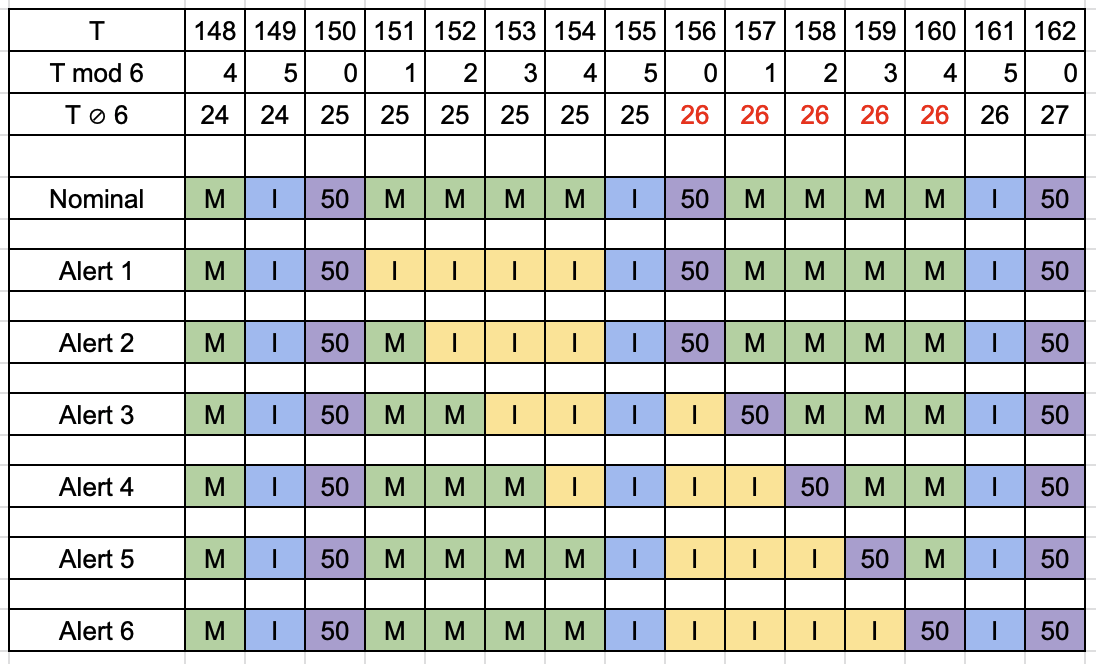
\includegraphics[width=0.5\linewidth]{fig/alertschedule.png}
				\caption{Conceptual diagram of how the counter scheme accommodates perturbations to the MT50 schedule. In the diagram, m means a standard message, and I means an integrity message. Integrity messages that would be sent on a nominal schedule are marked blue, and extra integrity messages during an alert are marked yellow. Note that $T \oslash 6$ does not change in the event of an alert message MT50 delay, as shown in red, so the Hash Path is preserved.}
				\label{fig: alert schedule}
			\end{figure}

			To assert the security of our scheme, it is essential that, in the event of an alert, any delayed MT50 sign the original messages corresponding to the loosely synchronized schedule.
			Concretely, in Figure~\ref{fig: alert schedule} in the row labeled Alert 6, (1) the MT50 of column 160 must sign the messages of columns 151 through 155, (2) the MT 50 of column 162 must sign the messages of columns 157 through 161, and (3) the non-MT50 message of column 156 remain unauthenticated.
			For the rows labeled alerts 3 through 6, the integrity messages of column 156 each remain unauthenticated.
			This is acceptable because those messages will only tell receivers not to use the service, and the surrounding integrity messages will be authenticated anyway.
			Without asserting this requirement, this security scheme becomes less secure.
			The security hinges on the loosely synchronized schedule, which is susceptible to a replay attack or a time-delay attack.
			If authenticated messages are occasionally sent after their agreed schedule, then the amount of replay delay required is occasionally reduced, and an adversary could spoof alerts to make such a replay attack easier.

	\subsection{TESLA Security} \label{sub:tesla_security}

		Previous work determined the appropriate security-level lengths under conservative adversary models\cite{Neish_Dissertation}.
		That work asserts that a TESLA Hash Point length of 115-bits and an HMAC length of 15-bits is sufficient to deter a supercomputer level attack over the time-between-authentication interval and assert a sufficiently low probability of success.
		In this work, we round these numbers up to the nearest base-2 number, 128 and 16, respectively.
		Increasing these lengths adds additional security-level padding.
		The primary reason for 128 Hash Point lengths is that MT51, as specified, has space for 128 bits.
		Section~\ref{sec:otar_design_methodology} discusses why 128 was selected to aid in the scheme's maintenance.
		The selection of 16-bit HMAC lengths follows our general strategy of 2-bit lengths, which aids the flexibility of the scheme, as discussed in Section~\ref{sub:metadata_design}.

		Until the Hash Point is released, the HMACs are indistinguishable from random bits.
		Given the security of the {\em salted} Hash Path, the probability that an adversary could forge a preimage Hash Point is $2^{-128}$.
		This probability is sufficiently low that it should not be expected to ever occur even with the support of vast computational resources.
		Given the desire to use the 128-bit Hash Path efficiently, see Section~\ref{sub:tesla_efficiency}, at a particular Hash Point time interval, we desire to authenticated many different pieces of information simultaneously (e.g., five messages per Hash Point, Section~\ref{sub:core_eph}).
		To do this securely, we must ensure that each piece of information authenticated with an HMAC has its own cryptographically independent HMAC key.
		This is the purpose of Equation~\eqref{eq: key}.
		Equation~\eqref{eq: key} takes the secure Hash Point and uses HMAC to derive a set of cryptographically independent keys by applying HMAC with (1) the Hash Point as the HMAC key field and (2) some {\em unique} identification information in the HMAC message field.
		In the specific case of Equation~\eqref{eq: key}, the HMAC message field includes the message time, the satellite PRN code, and the frequency.
		The time allows for a single Hash Point to authenticate the five messages individually since each message is sent at a different time.
		The PRN code allows all of the satellites to share the same Hash Path since each satellite has its own unique PRN code, and so forth with frequency.
		Our time, PRN code, and frequency band choices are arbitrary, except that our selection guarantees uniqueness: each message from each satellite from each band gets a cryptographically independent key to derive the HMAC.
		Any unique identifying information, such as a counter, would suffice to ensure the output of Equation~\eqref{eq: key} is cryptographically independent.

		Suppose the specifications of the previous paragraph were not met.
		An adversary could listen for any SBAS message and then broadcast that message four additional times before the next MT50 or forge the message as coming from another satellite.
		Hence, to assert authenticating security of a particular message from a particular satellite, the HMAC key must derive from the time, satellite source, and frequency.

		Since the Hash Point is not known to an adversary when the HMACs are released, the probability that an adversary can forge a 16-bit HMAC is $2^{-16}$.
		To provide adequate protection against forgery, we must specify a conservative forgery detection approach.
		For example, if any of the smaller HMACs fails the HMAC verification algorithm, the receiver must throw out all non-MT51 information from that particular SBAS satellite and restart collecting new SBAS data.
		While $2^{-16}$ is a relatively weak security level, this is sufficient for the SBAS context because (1) an adversary does not yet have access to the delay-released key nor an HMAC verification oracle (from the cryptography security context), and (2) any forgery detection immediately discards all prior SBAS data.
		A receiver must receive at least seven authenticated SBAS messages to obtain a useful navigation solution.
		The probability that an adversary could forge that many messages successfully is {}sufficiently small to meet the required security level.
		Another potential method to deter forgery is to require verification of two out of five of the signatures per MT50 before using any of that data.
		This decreases the probability of successful forgery to $2^{-32} < 10^{-9}$.		

		Our selection of SHA-256 for the Hash Path and HMAC generation is not necessarily required.
		We select SHA-256 because it is standard and widely used.
		We select HMAC-SHA-256, which calls SHA-256 as its primitive, to simplify the protocol.
		The widespread and straightforward use of SHA-256 aids in the continued security of the scheme.
		If the security SHA-256 is broken, it will be widely publicized and quickly deprecated for another hash function.
		Providers would need only replace the single function in their implementation and continue operation, much like the recent SHA-1 deprecation.

\section{OTAR Design Methodology} \label{sec:otar_design_methodology}

	The proposed design of MT51-B is fundamentally {\em modular}.
	The design of MT51-B serves only to deliver pseudorandom data so that its use can be flexible and recycled among different OTAR designs and applications that require delivery of pseudorandom data such as keys, signatures, and Hash Points. 
	Its purpose is to deliver large chunks of pseudorandom data to maintain the SBAS authentication scheme and the associated metadata on how the receiver should interpret that authenticating psuedorandom data.
	The same message definition delivers TESLA Hash Path Ends, level-2 keys, level-1-key decryption keys, and the authenticating psuedorandom data required to authenticate each.

	Our choice to allow 128-bits per MT51-B serves several purposes.
	We select 128 and 256-bit security level ECDSA keys since there exist standardized, secure elliptic curves at those security levels, and they are each divisible by 128.
	The public keys and derived signatures are twice and four times the security level length, respectively.
	These quantities are divisible by 128, meaning that there will be integer numbers of OTAR Payload Segments without wasted zero padding.
	Table~\ref{tab: psuedorandom lengths} shows how many messages are required to OTAR each of the key levels.
	Our selection could be modified to use the 192-bit level without modifying our scheme, since all of the 192-bit level data is also divisible by 128.
	The design is agnostic to the asymmetric scheme and is recycled for OTAR of the Hash Path Ends, expanding its use to the entire scheme's maintenance, not just the asymmetric portion.
	The proposed MT51-B standard would require no changes if a more efficient authentication scheme (e.g., EC-Schnorr), a quantum-secure scheme, or a different security level replaced the proposed asymmetric authentication scheme.
	The modular design also allows easy expansion of additional features described in Sections~\ref{sub:metadata_design} and~\ref{sub:core_eph} that may desirable to SBAS stakeholders.
		\begin{table}[H]
		\center
		\begin{tabular}{|c|c|c|c|c|} \hline
			Key Level & Security Level & Public Key Length & OTAR Bit Requirement & MT51-Bs Req. \\ \hline
			    1 & 256 & 512 &  128 & 1 \\ \hline
			    2 & 128 & 256 & 1280 & 10\\ \hline
			TESLA & 128 & 128 &  640 & 5 \\ \hline
		\end{tabular}
		\caption{Table that delineates the number of MT51-Bs required to complete a single OTAR for a specific key. Level-1 keys require only the 128-bit AES decryption key, hence a single MT51-B. Level-2 keys require 256-bit key, and 1024 bits of authenticating psuedorandom data (twice the Level-1 public key length), hence 1280 bits and 10 MT51-Bs. TESLA Hash Path Ends require 128-bit Hash Point and 512 bits of authenticating psuedorandom data (twice the level-2 public key length), hence 640 bits and 5 MT51-Bs. Each unique MT51-B is required to OTAR.}
		\label{tab: psuedorandom lengths}
	\end{table}

	MT50 and MT51 are agnostic to the asymmetric cryptographic security scheme and hash function primitives.
	When the security of a primitive becomes compromised, the SBAS MT scheme need not change.
	Providers and receivers will have to change the primitives used modularly.
	Since MT51-B provides 128-bits of authenticating pseudorandom data per message, and standardized cryptographic primitive lengths are, generally, integer factors of 128, changes to the scheme would increase or decrease the number of segments required to transmit information.
	If the security of the 128-bit truncated SHA-256 is ever compromised, SBAS could double the Hash Point length space without affecting the MT50 frequency as follows.
	Suppose the Hash Point space is the set of 256-bit integers, like the untruncated SHA-256.
	Each MT50 will transmit half of a Hash Point, and each HMAC key will derive from two consecutive MT50 messages.
	This increases the time-between authentication by a few seconds; however, it doubles the Hash Path security and maintains the loss-tolerant properties.

	\subsection{MT51-B Metadata Design} \label{sub:metadata_design}

		Within the authenticating psuedorandom data metadata, we specify the inclusion of a Germane and Authenticating Key hash.
		Since the payload is pseudorandom, metadata must exist so that the receiver can associate the unique MT51-B payloads.
		Any identifying feature would suffice, such as the ordered key number, rolling over every $2^{16} = 65536$ keys.
		However, the use of hash on the entire key provides additional features.
		The key schedule need not be rigid, linear, or sequential.
		Provider and CA can maintain several redundant level-2 and level-1 keys, respectively.
		Multiple keys, perhaps managed in isolation by Provider and CA, could provide redundant security.
		Provider would need to be careful that two unexpired keys do not share the same 16-bit identifying hash; however, this would be a rare event, and Provider would need only randomly draw another key in that event.

		SBAS Providers could mutually broadcast each other's Hash Path Ends and key maintenance to promote service continuity; hence, we included the SBAS Service Provider ID in the metadata.
		SBAS Providers would not need access to each other's secrets; they would only act as a repeater.
		Whereas Section~\ref{sub:mt51_schedule_frequency} discusses higher MT51-frequency to support the local SBAS authentication from cold receiver start, this feature would be low frequency to support the local Provider schedule.
		Having Providers broadcasting each other keys at low frequency would aid in the TFAF when transferring to a new SBAS Provider.
		For example, consider two adjacent SBAS systems, WAAS and EGNOS, and an aircraft traversing from Europe to North America.
		It takes several hours for aircraft to make this journey.
		If EGNOS broadcasts the WAAS keys once an hour, any westward aircraft will receive the necessary WAAS keys to operate before reaching North America, decreasing the WAAS TFAF to zero. 
		At a minimum, SBAS Providers could broadcast adjacent SBAS Providers' keys.
		Without this feature, when an aircraft enters a new SBAS service volume the first time of the week (or 10 or 100 weeks), it must act as a cold-start receiver for to the amount of time required to get the Authentication Stack, as specified in Section~\ref{sub:mt51_schedule_frequency}.

		Spare bits in the authenticating psuedorandom data metadata could accommodate other features.
		These include scheme hyperparameters, such as the choice of a hash function or key or HMAC length.
		MT51-B messages could authenticate specific messages, identified by 16-bit hashes, immediately with ECDSA.
		If keys are ever compromised, MT51-B could also disseminate key revocations.
		A revocation MT51-B would include eight 16-bit hashes of the affected keys and would only need to be broadcast until the keys are retired under standard procedure.
		Since each broadcast of an MT51-B is accompanied by a germane expiration time, Provider can arbitrarily shorten the applicability of a particular key by rebroadcasting the MT51-B with a different expiration time, noting the assumption that receivers actually receive and record that updated broadcast and that the Hash Path salt is not disrupted, see Section~\ref{subsub:ecdsa_salt}.
		Receivers would need to remember key expiration time changes and key revocations, and receivers that did not receive that update would remain vulnerable.
		If Provider can re-sign data, the metadata must include a parameter that identifies that particular authentication.
		This is because without the germane key hash, authenticating key hash, segment number, and authentication instance number, each segment of psuedorandom data cannot be associated because they are pseudorandom.
		Furthermore, MT51-B could manage other authentication schemes, such as an authentication scheme adopted by GNSS, see Section~\ref{sub:core_eph}.
		A GNSS authentication, especially one built on TESLA, would save bandwidth by deferring the GNSS scheme's maintenance to SBAS.

		There are many features that the scheme's modularity can accommodate; however, if SBAS stakeholders do not want any of these features, then the spare meta bits could also be used to aid in resistance to message loss.
		Providers could add redundant HMACS to the MT51-B message to redundantly authenticate messages to alleviate MT50 message loss.
		Moreover, the delivery of 128-bits of authenticating psuedorandom data could be augmented with fountain codes \cite{gnss_fountain_codes}.
		Fountain Codes (1) increase the reliability of delivering MT51 messages and (2) decrease the number of transmitted messages required for an authenticated first fix.
		The selection of 128-bits aids in the scheme's efficiency since all the data is integrally divisible by 128.
		Special care can ensure that using fountain codes in the spare bits to augment those 128-bits would not change the integrally divisible property and maintain efficiency.
		Moreover, as features discussed are discards, SBAS Providers could use MT51-A.
		The balance between MT51-A and MT51-B is discussed in Section~\ref{sec: MT51 balance}.

	\subsection{Core Constellation Ephemerides Authentication} \label{sub:core_eph}

		Another feature accessible with this schemes modularity is authenticating navigation messages from GNSS systems.
		GNSS data messages have limited bandwidth and must maintain backward compatibility.
		MT51-B provides a natural pathway to authenticate GNSS data with the 128-bit payload and spare meta-data bits.
		Table~\ref{tab: meta-data} already provides the required metadata designations: (1) the germane core constellation system, (2) the type of authenticating psuedorandom data, and (3) the authenticating psuedorandom data segment number.
		However, the payload should be modified to accommodate the realistic operation.

		One could use a single MT51-B payload to authenticate the entire set of ephemerides with a single 128-bit HMAC; however, this would not work for realistic receivers.
		In order to use a single 128-bit HMAC, the receiver must have the entire set of ephemerides.
		This is unrealistic since receivers will not receive the set of ephemerides of satellites outside its view.
		Therefore, like the MT50 design, we suggest that the 128-bit payload be split into eight 16-bit payloads, as shown in Table~\ref{tab: nma}.
		Each 16-bit HMAC within the MT51-B payload corresponds to a specific satellite's broadcast ephemerides, and the MT51-B metadata informs the receiver which satellites correspond to the payload HMACs.
		By splitting the payload into smaller HMACs, the receiver need not have the entire set of ephemerides to authenticate individual satellites.

		\begin{align}
			k_j &= \textrm{HMAC}(p^P_i, t_j || \textrm{PRN}_\textrm{SBAS} || \textrm{Frequency}_\textrm{SBAS} || \textrm{SVN}_\textrm{Core} \label{eq: ephemerides key}) \\
			s_j &= \textrm{HMAC}(k_j, \textrm{Ephemeride}_{\textrm{SVN}}) \label{eq: ephemerides signature}
		\end{align}

		\begin{table}
			\center
			\begin{tabular}{|c|c|c|c|c|c|c|c|c|c|} \hline
				Metadata, etc & HMAC1 & HMAC2 & HMAC3 & HMAC4 & HMAC5 & HMAC6 & HMAC7 & HMAC8 & CRC \\ \hline
				98 & 16 & 16 & 16 & 16& 16 & 16 & 16 & 16 & 24 \\ \hline
			\end{tabular}
			\caption{Bit allocation proposed for a particular MT 51 to authenticate the entire set of ephemerides at 250 bits per message with 128-bit payload.}
			\label{tab: nma}
		\end{table}

		There are two important security details.
		First, like with MT50, if any of one of the HMACs return unauthenticated, then all of the entire set of ephemerides data must be thrown out.
		Second, the HMACs derive from a cryptographically independent key derived from a TESLA Hash Point, like as described in Section~\ref{sub:tesla_security}.
		Equations~\eqref{eq: ephemerides key} and~\eqref{eq: ephemerides signature} use the sending time $t_j$, the SBAS PRN and frequency, and the core constellation satellite vehicle number.

		SBAS could authenticate the broadcast ephemerides of every satellite globally, and the receiver can draw from the entire set of HMACs the few in view of the receiver.
		The metadata segment number informs the receiver from which set of eight satellites the HMACs derive.
		For GPS, this would mean four of these MT51-Bs.
		However, MT1 and MT31 already provide an issues-of-data mask of the 92-most relevant satellites currently under correction of a particular SBAS.
		Therefore, we propose that the order of the eight HMACs correspond to the order prescribed in the issues of data already provided to the receiver.
		The issue of data index, either the IODP or IODM, must be placed in the unused sections of the metadata, and the metadata segment number field would determine the relevant eight, in order, among the set of 92.
		Since the issue of data index requires only two bits, SBAS could use the unused German Key Hash, German Key Expiration, and Authenticating Key Hash to send 12 HMACs per MT51-B.
		Alternatively, one could define a new message type that delivers 13 HMACs, the issue of data index, and the segment number.

	\subsection{MT50 Redundant Authentication} \label{sub:mt50_redundant_authentication}

		MT51 messages are self-authenticating, resulting from the use of ECDSA.
		Upon receipt of the entire Authentication Stack, the receiver can assert authenticity to the level-1 key maintained by CA.
		However, the MT51 messages are among the SBAS messages authenticated via TESLA and MT50.
		If the receiver has an ECDSA-verified Authentication Stack, which can authenticate the bulk of SBAS messages via MT50, the receiver can use TESLA to verify the next Authentication Stack when delivered via MT51.
		Concretely, a receiver can assert the authenticity of the next Hash Path End without awaiting the associated authenticating psuedorandom data since an HMAC in the following MT50 will assert authenticity down to the current Hash Path End through the current level-1 key.
		In Section~\ref{sub:mt51_schedule_frequency}, we suggest that the next Authentication Stack be rebroadcasted each hour.
		The ECDSA-based and TESLA-based authentication of the next Authentication Stack is redundant to a receiver with an authenticated fix.
		Therefore, an argument can be made that is the hour-long frequency to broadcast the next Authentication Stack does not add to the scheme.
		Alternatively, MT50s could not authenticate MT51s and instead authenticate messages redundantly.
		These considerations will ultimately depend on the manufacturer's implementation preference and whether the logic should be incorporated into the process.
		To avoid implementation errors that could potentially serve as exploits in the authentication scheme, we suggest that, given stakeholder agnosticism, the simplest version be selected.
		We feel that the scheme delineated above, where MT51 data is redundantly authenticated with MT50, is the simpler scheme.

	\subsection{MT51-B Schedule Frequency} \label{sub:mt51_schedule_frequency}

		As mentioned earlier, we propose that the cryptoperiod of the level-1, level-2, and TESLA Hash Paths be 100, 10, and 1 week, respectively.
		Our selections are arbitrary.
		However,  any choice must meet minimum security requirements associated with the required computational time to guess the keys exhaustively.
		Upon cold receiver startup, we desire that the TFAF be reasonably short.
		Therefore, the Authentication Stack must be sent periodically over their use.
		From Table~\ref{tab: psuedorandom lengths}, a complete Authentication Stack requires 16 MT51s. 
		We propose that Provider broadcast the current Authentication Stack every 5 minutes so that a cold-start receiver achieves the first authenticated fix in 5 minutes, assuming no message loss.
		This requirement would require that a message from the set of 16 unique MT51-Bs be transmitted 1 out of every 18 messages, rounded up.
		With multiple geostationary satellites and frequencies, the satellites can broadcast the unique MT51s out of phase to decrease the authenticated first fix time as mentioned in Section~\ref{sub:tesla_efficiency}.

		Furthermore, the next keys, applicable immediately upon expiration of the current keys, must be sent well before their actual use for a seamless transition as keys expire.
		To protect a specific new key's security, it would be prudent to only send that new key just before use.
		For instance, we suggest Provider send the next 100-week level-1 key repeatedly beginning five weeks before its actual use and send the next 10-week level-2 and 1-week TESLA Hash Path End 1 week before its actual use.
		To show how little this consideration affects the MT51-B SBAS bandwidth, if a Provider sent the next Authentication Stack once every hour, together with the current Authentication Stack once every 5 minutes, Provider would need to send a message from the set of 32 unique MT51s 1 out of every 17 messages, rounded up.
		This assumes that each OTAR Payload Segment of the Authentication Stack is broadcast at the same frequency, as a base line.
		Since some sections of the Authentication Stack change less frequently, further optimization could balance TFAF with the likelihood that receivers are off more than for 1 week, 10 weeks, or 100 weeks.
		For instance, the slowly varying OTAR Payload Segments could be broadcast once ever 15 minutes, and the weekly varying OTAR Payload Segments every 2 minutes.

		We note that it is not required that Providers and receivers stick to a set schedule for the key periods or the Hash Paths.
		As discussed before, the MT51-B metadata and modularity afford flexibility in expirations of particular keys and the agreed schedule for expirations.
		Moreover, switching Hash Paths by Provider without warning does not add computational complexity to receiver verification.
		Each Hash Point is a hash, and hashes have constant-time look-up computational complexity, as seen in Algorithm~\ref{alg: TESLA receiver}.
		This means if Provider were to switch Hash Paths without warning, the receiver would need only one additional computation to check that the new Hash Point is the preimage to another ECDSA-verified Hash Path End.
		This means that SBAS could incorporate unscheduled or stochastic Hash Path switches, provided the appropriate MT51s are sent in advance, noting that the MT51s only specify Hash Path End expirations and not their actual use time.
		If stakeholders elect not to have a rigid Hash Path schedule, a maximum Hash Path length upper bound must be specified so that receivers do not get stuck in an infinite hashing loop attempting to hash back down to an ECDSA-authenticated Hash Path End.

		The selection of the level-1 cryptoperiod, level-2 cryptoperiod, and Hash Path length pose trade-offs among SBAS stakeholders.
		With a very long Hash Path, aircraft are less likely to be in a state where they do not have the current Hash Path End via MT51 since the Hash Path End expires less often.
		Upon startup after a shutdown less than the Hash Path End cryptoperiod, (1) receivers need not await delivery of an updated Authentication Stack via MT51, and (2) receivers must accommodate a more intense startup hashing operation to hash the current MT50 Hash Point to the authenticated Hash Path End.
		With a very short Hash Path (e.g., a Hash Path cryptoperiod of 1 day), after a receiver shutdown, receivers will more likely be in a state of missing part of the Authentication Stack since those missing parts expired while the receiver was shut down, but the shorter Hash Path will mean less hash processing at startup.
		These considerations become especially germane for aircraft that traverse different SBAS service volumes periodically.
		For instance, consider aircraft that make transatlantic regularly, which, when outside a specific service volume, behave as a shutdown receiver.
		Our selection from this Section~\ref{sub:mt51_schedule_frequency} was to accommodate a short time of the first fix.
		With a longer Hash Path, as flights cross service volumes, the more likely the TFAF will be bounded by receiver computational hash capability instead of being bounded by MT51 delivery schedule.

	\subsection{MT51-A/B Balance} \label{sec: MT51 balance}

		A final MT51 design must accommodate all the features relevant to SBAS stakeholders while maintaining the KPIs.
		The most relevant KPI for this discussion is TFAF, since more features requires more metadata, which increases the number of unique MT51s required to OTAR.
		We propose MT51-B because we make the claim that the minimum MT51 OTAR Payload Segment size acceptable is 128-bits, given the conveniences discussed in other sections, allowing us to specify a maximum metadata.
		We propose MT51-A to (1) acknowledge there are other ways of constructing the MT51 metadata that remove definition redundancy and spare bits and (2) specify the minimum metadata.
		For instance, the SBAS Provider could identify keys by their expiration time, removing the need for the Germane and Authenticating Key Hashes in the metadata; however, this would disallow parallel and redundant key management.
		As SBAS Stakeholders discuss their desires, the metadata will become more or less crowded (noting even MT51-B has some spare bits).
		Therefore, we offer a couple of suggestions on how to reason about balancing the design while maintaining the schemes modularity, simplicity, and flexibility.

		First, as features are removed, rather than shifting bit allocations from the metadata to OTAR Payload Segment, SBAS Providers could instead replace metadata bits with fountain codes.
		This suggestion would (1) maintain the MT51's integer-division property on the authenticating psuedorandom data ensuring there is no wasted zero-padding on the delivered data, and (2) add loss-tolerant properties of MT51.
		Fountain codes can arbitrarily occupy spare bits.
		Second, MT51 could have a 192-bit OTAR Payload Segment length.
		While this will not maintain the integer-division property always, this should limit any zero padding to 64-bits.
		For instance, 18 MT51-Bs deliver 2304-bits, which can also be delivered with 12 MT51s with 192-bits of OTAR Payload Segment lengths.
		An example Authentication Stack of this exact length would the same as that of Table~\ref{tab: psuedorandom lengths} with the following modifications: (1) using AES-256 to encrypt level-1 keys and (2) having a separate TESLA salt MT51.
		This would leave up to 24-bits of metadata per message and there would be several OTAR Payload Segments that contain multiple types of psuedorandom data (like with MT51-A). 
		Third, all of the meta data required could be placed in a single MT51 OTAR Payload Segment; i.e., a specific OTAR Payload Segment could contain all the meta data required to interpret the Authentication Stack.
		We implore the SBAS Stakeholders to have a future-proofing mindset to allow for considerations that may be needed decades in the future.
		Cryptographic primitives will break and need to be replaced; Quantum-computer resistant algorithms may be needed.
		And the best way to maintain a future-proof mindset is to make MT51 agnostic to the data its delivering and expandable to any future psuedorandom data delivery required.

\section{TESLA Time Synchronization} \label{sec:tesla_time_synchronization}

	The HMAC keys authenticating all SBAS messages with HMACs derive from the Hash Path delay-released on an assumed schedule.
	Therefore, it is critical to the Hash Path security that Provider and the receiver are loosely time-synchronized.
	Loosely time-synchronized means that the receiver has a sufficient, externally-trusted time to reject HMACS after the release of the associated Hash Point.
	This poses a catch-22 to aircraft that use an isolated GNSS receiver since GNSS provides the time.
	GNSS ranging signals allow receivers to derive an accurate, atomic-clock-synchronized time which is certainly accurate enough to support the delay-release schedule.
	There are ways from the prior art by which receivers can establish trust in GNSS ranging signals\cite{Psiaki2016, Fernandez-Hernandez2018}; however, GNSS ranging signals are not yet rigorously authenticated with cryptography.

	To break SBAS security by breaking the loosely time-synchronized assumption, an adversary must spoof the receiver time by delaying the receiver time.
	In our case, this delay is 7 seconds.
	If the receiver clock were 7 seconds behind Provider's clock, an adversary listening to Provider could note the delay-released Hash Point, derive the keys, and generate forged HMACs.
	The longer the delay, the more HMACs an adversary can forge.
	Naively, one could ensure that the receiver does not allow 7-second jumps of time to mitigate; however, this strategy would not work with a creeping Replay Attack, the worst-case attack model we examine in this work.
	In a creeping Replay Attack, an adversary listen and replays the GNSS and SBAS signals but incrementally delay them slowly enough to avoid detection by the receiver.
	There are several mitigation strategies to mitigate the creeping Replay Attack.

	The first is to use its onboard clock to evaluate a spoofed-time hypothesis.
	The prior art has explored how to use clock tolerances to generate and use tolerance bounds to assert clock trust\cite{time_sync_paper}.
	We have explored a few methodologies to fuse GNSS and onboard clock to evaluate whether a receiver is actively in a creeping Replay Attack, such as Pearson hypothesis tests and Kalman-filter-based hypotheses tests.
	The explicit hypothesis methodologies and their evaluation are left for other work.
	These strategies can detect a creeping Replay Attack before the 7-second breakage boundary, provided the creeping delay rate is faster than the uncertainty bound of the onboard clock.
	For instance, a consumer quartz clock oscillator will gain or lose on the order of 15 seconds a month.
	This means that any hypothesis test that exclusively uses the onboard clock to estimate an authentic time is information-bound to 15 seconds per month.
	Aircraft caretakers and airport security officials could consider implementing procedures that guarantee that the aircraft receiver periodically receives a trusted GNSS and SBAS signals, such as while taxiing at an airport where security officials ostensibly monitor for spoofed signals and jamming.
	Operators would need to communicate with the receiver that the current estimate can be trusted to reset the information-bound consideration.
	Receiver manufacturers could invest in more accurate clocks to tie these periodical time-trust events to periodic maintenance.

	The second is to compare to an external-to-GNSS, trusted time.
	Every day, billions of devices establish time via rigorous cryptographic authentication via the internet.
	This system addresses tangential security concerns such as internet-based banking, and it works well since the internet does not have the SBAS bandwidth limitation.
	A receiver could compare its own time to an internet-based time or a cellular-based time.
	This comparison need only bound the GNSS-based time: the receiver can still utilize the accurate time derived from the GNSS positioning regression time, but check that it matches the internet-based time within a bound such as one second.
	This internet or a data-based time can be rigorously authenticated with cryptographic authentication according to the standard of the medium.
	The original TESLA protocol provides a secure time-synchronization procedure: Provider would establish an internet server to accept and operate on receiver-generated nonces that would work within the secure Hash Path\cite{perrig2005timed}.
	Our choice to use the word {\em compare} is intentional to address the concern about allowing external inputs regarding time into the isolated SBAS receiver.
	This comparison is achievable without exposing the receiver's time to archetype hacking strategies.
	Other strategies would also alert the pilot that the SBAS time is not trusted, such as incorporating the GNSS time estimate into the Air Traffic Control Radar Beacon System.
	If the beacon-broadcasted time were more than 7 seconds behind the trusted time on the ground, then ground services could alert the aircraft of the discrepancy.

	Since the ranging signal remains unauthenticated via rigorous methods established with cryptography, SBAS must take a nuanced approach to assert the loosely time-synchronized assumption.

\section{Full Stack Simulation AND KPIs} \label{sec:full_stack_simulation}

	To examine the efficacy of this scheme, we implemented a full-stack simulation of this scheme in MAAST.
	By full-stack simulation, we mean the MAAST Matlab implementation called the secure com.sun.security.auth java package to (1) simulate actual SBAS message transmission with ECDSA and TESLA routines asserting authentic messages and (2) testing that verifies that forged messages are detected.
	At the time of publication, the scheme in its entirety herein was implemented except (1) the hash path salt, (2) the PRN concatenation operation allowing multiple satellites, (3) pre-stored encrypted level-1 public keys.
	These features do not materially affect the results' outcome because we took special care to ensure that the simulated scheme had the same number of unique messages per Authentication Stack.
	Implementing these features is left to future work after feedback from the SBAS stakeholders on this work.

	With MAAST, we modified the message scheduler to (1) send MT50s at a cadence of one in six messages and (2) send MT51s whenever the schedule allowed an opening.
	Given the current use of the SBAS message schedule, MT51s were sent more frequently than the requirement specified above at one in seventeen messages.
	Therefore, among our simulations, TFAF occurred usually within one minute, and if not, just outside one minute.
	The TFAF is less than our requirement from Section~\ref{sub:mt51_schedule_frequency} because the simulated Provider sent the 16 unique messages within open slots of the SBAS schedule.
	Therefore, our simulation indicates that SBAS availability and continuity are not affected by this authentication scheme.

\section{Conclusion} \label{sec:conclusion}

	By delineating and establishing the cryptographic authentication security and showing that it does not materially affect the performance of SBAS, we show that this scheme is a viable solution to appending cryptographic authenticity to SBAS.
	This scheme merely appends two message types to the schedule, meaning it does not require removing power from the I-channel to support a Q-channel strategy.
	The scheme is immediately backward compatible because older receivers can ignore the new message types.
	Given the reasonable use of onboard clocks, external clocks, and maintenance patterns, we assert the existence of reasonable, nuanced strategies to mitigate attacks against the lose time-synchronized assumption required by TESLA.
	Given that we can achieve authentication with just two MTs on the I-channel, we believe this scheme, or something similar, is the best way to achieve SBAS authentication.

\bibliographystyle{ieeetr}
\bibliography{references}



\end{document}